\chapter{Analyse et sp\'{e}cification des besoins}
\label{chap:analyse}

\vspace{2cm}

\noindent\textbf{\Large Plan}

\vspace{0.5cm}
\noindent\rule{\textwidth}{0.4pt}
\vspace{0.3cm}

\begin{list}{}{\setlength{\leftmargin}{1.5cm}\setlength{\itemsep}{6pt}}
  \item \textbf{1} \hspace{0.3cm} Analyse des besoins \dotfill \pageref{sec:analyse}
  \item \textbf{2} \hspace{0.3cm} Identification des besoins \dotfill \pageref{sec:identification}
  \item \textbf{3} \hspace{0.3cm} Sp\'{e}cification des besoins \dotfill \pageref{sec:specification}
  \item \textbf{4} \hspace{0.3cm} Cadre m\'{e}thodologique \dotfill \pageref{sec:cadre}
  \item \textbf{5} \hspace{0.3cm} Conclusion \dotfill \pageref{sec:conclusion}
\end{list}

\vspace{0.3cm}
\noindent\rule{\textwidth}{0.4pt}

\newpage

\section*{Introduction}

Ce chapitre est consacr\'{e} \`{a} l'analyse de l'existant ainsi qu'\`{a} la sp\'{e}cification des besoins n\'{e}cessaires pour atteindre les objectifs du projet. Dans un premier temps, nous pr\'{e}sentons l'\'{e}tude de l'existant et la solution envisag\'{e}e. Ensuite, nous d\'{e}finissons les diff\'{e}rents acteurs du syst\`{e}me ainsi que leurs besoins. Enfin, nous d\'{e}crivons la m\'{e}thodologie adopt\'{e}e, en d\'{e}taillant le backlog produit et la planification des sprints.

\section{Analyse des besoins}
\label{sec:analyse}

Cette section pr\'{e}sente l'analyse du processus actuel de gestion des demandes dans le secteur des pi\`{e}ces de rechange automobile, ainsi qu'un aper\c{c}u des solutions num\'{e}riques existantes.

\subsection{Pr\'{e}sentation de l'organisme d'accueil}

\textbf{Insy2s} est une entreprise de services du num\'{e}rique (ESN) sp\'{e}cialis\'{e}e dans le conseil, le d\'{e}veloppement logiciel et l'int\'{e}gration de solutions digitales. Elle intervient dans plusieurs secteurs d'activit\'{e} tels que l'assurance, la finance, l'industrie et les t\'{e}l\'{e}communications. Elle compte une \'{e}quipe d'ing\'{e}nieurs hautement qualifi\'{e}s aux profils vari\'{e}s, ce qui refl\`{e}te une grande diversit\'{e} de comp\'{e}tences et de parcours.

\begin{table}[H]
\centering
\caption{Fiche signal\'{e}tique de l'organisme d'accueil}
\label{tab:fiche}
\begin{tabular}{|p{5cm}|p{8cm}|}
\hline
\textbf{Propri\'{e}t\'{e}} & \textbf{Valeur} \\
\hline
Raison sociale & Insy2s \\
\hline
Secteur d'activit\'{e} & Services du num\'{e}rique (ESN) \\
\hline
Domaines d'intervention & Assurance, Finance, Industrie \\
\hline
Services propos\'{e}s & Conseil, D\'{e}veloppement, Int\'{e}gration, IA \\
\hline
Technologies & Java, Spring Boot, React, Flutter, Python \\
\hline
\end{tabular}
\end{table}

\subsection{\'{E}tude du processus actuel de gestion des demandes}

Le secteur des pi\`{e}ces de rechange automobile en Tunisie g\`{e}re quotidiennement un volume \'{e}lev\'{e} de demandes clients provenant de canaux h\'{e}t\'{e}rog\`{e}nes --- t\'{e}l\'{e}phone, email et visite en agence. Le traitement de ces demandes repose actuellement sur un circuit essentiellement manuel, dont les limites structurelles impactent directement la qualit\'{e} du service et la productivit\'{e} de l'entreprise.

\indent Lorsqu'un client contacte l'entreprise, l'op\'{e}rateur r\'{e}ceptionne l'appel sans aucun support num\'{e}rique d\'{e}di\'{e}. Les informations communiqu\'{e}es sont consign\'{e}es manuellement sur papier ou dans un tableur, ce qui expose le processus \`{a} des erreurs de saisie et \`{a} une lenteur consid\'{e}rable. L'op\'{e}rateur s'appuie ensuite sur son exp\'{e}rience personnelle pour \'{e}valuer les conditions de garantie applicables, puis formule une d\'{e}cision sans outil de scoring ni m\'{e}canisme de tra\c{c}abilit\'{e}. La r\'{e}ponse est finalement transmise oralement au client, sans archivage formel de la d\'{e}cision prise.

\paragraph{Critique de l'approche actuelle}

L'analyse de ce processus r\'{e}v\`{e}le un ensemble de dysfonctionnements \'{e}troitement li\'{e}s, qui se renforcent mutuellement et fragilisent l'efficacit\'{e} globale du service.

\indent L'absence d'outils num\'{e}riques d\'{e}di\'{e}s constitue la premi\`{e}re limite majeure. Elle contraint les op\'{e}rateurs \`{a} saisir manuellement chaque information, ce qui g\'{e}n\`{e}re des erreurs de saisie fr\'{e}quentes et allonge consid\'{e}rablement la dur\'{e}e de traitement de chaque dossier. Cette lenteur est d'autant plus probl\'{e}matique qu'elle s'accompagne d'une fragmentation des donn\'{e}es~: sans syst\`{e}me centralis\'{e}, les informations relatives aux clients et aux demandes sont dispers\'{e}es entre diff\'{e}rents supports (papier, tableurs, m\'{e}moire des agents), rendant leur consultation particuli\`{e}rement laborieuse.

\indent \`{A} ces difficult\'{e}s op\'{e}rationnelles s'ajoute une absence totale de tra\c{c}abilit\'{e}. Sans historique num\'{e}rique des \'{e}changes et des d\'{e}cisions, il devient impossible de justifier les choix effectu\'{e}s en cas de litige ou d'en assurer un suivi qualit\'{e} rigoureux. Cette lacune est directement aggrav\'{e}e par la subjectivit\'{e} inh\'{e}rente au processus d\'{e}cisionnel~: les conditions de garantie \'{e}tant \'{e}valu\'{e}es de mani\`{e}re individuelle par chaque op\'{e}rateur, le traitement des dossiers manque de standardisation et g\'{e}n\`{e}re des in\'{e}galit\'{e}s entre les clients.

\indent Enfin, la d\'{e}pendance totale \`{a} l'expertise individuelle de l'op\'{e}rateur, conjugu\'{e}e \`{a} l'absence d'aide \`{a} la d\'{e}cision, ralentit le traitement et augmente le risque d'erreurs. Il en r\'{e}sulte un temps moyen de traitement estim\'{e} \`{a} plus de quinze minutes par dossier, ce qui peut entra\^{i}ner une perte de r\'{e}activit\'{e} et une insatisfaction client susceptible, selon les donn\'{e}es sectorielles, de conduire au changement de prestataire.

% === PARTIE 2 : Solutions existantes + Besoins ===

\subsection{\'{E}tude des solutions de gestion existantes}

Aujourd'hui, de nombreuses solutions num\'{e}riques existent pour optimiser le processus de gestion des demandes clients en entreprise. Apr\`{e}s une analyse approfondie du march\'{e}, nous avons retenu trois plateformes de r\'{e}f\'{e}rence dans ce domaine~: Zendesk, Freshdesk et Salesforce Service Cloud.

\indent \textbf{Zendesk} est une plateforme de service client destin\'{e}e aux entreprises souhaitant centraliser et automatiser la gestion de leurs demandes. Elle propose une exp\'{e}rience omnicanale couvrant l'email, le t\'{e}l\'{e}phone, le chat et les r\'{e}seaux sociaux \cite{zendesk}. Depuis 2023, Zendesk int\`{e}gre des agents IA (Zendesk AI) capables de r\'{e}pondre automatiquement aux demandes via WhatsApp et d'autres canaux de messagerie. Toutefois, les fonctionnalit\'{e}s IA avanc\'{e}es sont r\'{e}serv\'{e}es aux plans sup\'{e}rieurs (\`{a} partir de 115~\$/agent/mois), et la plateforme ne propose ni moteur de r\`{e}gles m\'{e}tier configurable ni option d'h\'{e}bergement local.

\indent \textbf{Freshdesk} est une solution de helpdesk digital qui permet aux entreprises de g\'{e}rer efficacement leurs tickets de support \cite{freshdesk}. Freshdesk int\`{e}gre Freddy AI, son moteur d'intelligence artificielle, qui permet la suggestion automatique de r\'{e}ponses et la classification des tickets. Cependant, la transcription automatique des appels vocaux n'est pas nativement disponible et requiert l'int\'{e}gration de services tiers. Il n'existe pas non plus de moteur de r\`{e}gles m\'{e}tier configurable visuellement par un utilisateur non technique.

\indent \textbf{Salesforce Service Cloud} est une plateforme CRM compl\`{e}te int\'{e}grant des outils avanc\'{e}s de gestion de la relation client \cite{salesforce}. Sa composante IA, Einstein AI, offre des fonctionnalit\'{e}s substantielles~: transcription et r\'{e}sum\'{e} automatique des appels, g\'{e}n\'{e}ration de r\'{e}ponses personnalis\'{e}es et classification automatique des cas. N\'{e}anmoins, ses capacit\'{e}s restent li\'{e}es \`{a} l'\'{e}cosyst\`{e}me Salesforce --- les mod\`{e}les IA sont pr\'{e}-entra\^{i}n\'{e}s sur des donn\'{e}es CRM g\'{e}n\'{e}riques et ne peuvent pas int\'{e}grer un moteur de r\`{e}gles m\'{e}tier sp\'{e}cifique \`{a} un secteur d'activit\'{e}. Son co\^{u}t est particuli\`{e}rement \'{e}lev\'{e}.

\indent Pour mieux comparer ces trois solutions, le tableau~\ref{tab:comparaison} synth\'{e}tise leurs caract\'{e}ristiques au regard des besoins sp\'{e}cifiques identifi\'{e}s pour notre projet.

\begin{table}[H]
\centering
\caption{Comparaison entre les solutions existantes}
\label{tab:comparaison}
\begin{tabular}{|p{3.5cm}|p{3cm}|p{3cm}|p{3.5cm}|}
\hline
\textbf{Crit\`{e}res} & \textbf{Zendesk} & \textbf{Freshdesk} & \textbf{Salesforce} \\
\hline
Gestion multicanale & Oui (email, t\'{e}l., chat) & Oui (email, t\'{e}l.) & Oui (complet) \\
\hline
Transcription IA & Non & Non & Partiel (Einstein) \\
\hline
Moteur de r\`{e}gles m\'{e}tier & Non & Non & Non \\
\hline
Aide \`{a} la d\'{e}cision IA & Non & Non & Partiel (Einstein AI, non sp\'{e}cifique au domaine) \\
\hline
Chatbot int\'{e}gr\'{e} & Partiel (Zendesk AI) & Partiel (Freshbot) & Partiel (Einstein Bot) \\
\hline
Co\^{u}t & \'{E}lev\'{e} & Moyen & Tr\`{e}s \'{e}lev\'{e} \\
\hline
H\'{e}bergement local & Non & Non & Non \\
\hline
Adapt\'{e} au secteur auto & Non & Non & Non \\
\hline
\end{tabular}
\end{table}

\indent Bien que ces outils apportent des solutions int\'{e}ressantes, y compris certaines fonctionnalit\'{e}s de chatbot (Zendesk AI, Freshbot) et d'IA partielle (Salesforce Einstein), ils restent g\'{e}n\'{e}riques et ne r\'{e}pondent pas pleinement aux besoins sp\'{e}cifiques du secteur des pi\`{e}ces de rechange automobile. Aucune de ces plateformes ne combine la transcription automatique des appels, un moteur de r\`{e}gles m\'{e}tier configurable avec versioning et une aide \`{a} la d\'{e}cision par intelligence artificielle adapt\'{e}e au domaine. De plus, aucune n'offre la possibilit\'{e} d'h\'{e}bergement local, essentielle pour la confidentialit\'{e} des donn\'{e}es. Ce constat justifie la conception d'une solution sur mesure.

\subsection{Solution souhait\'{e}e}

Face aux difficult\'{e}s constat\'{e}es dans l'approche actuelle, et au constat que les solutions existantes du march\'{e} ne r\'{e}pondent pas pleinement aux besoins sp\'{e}cifiques de l'entreprise, la solution souhait\'{e}e vise \`{a} optimiser l'exp\'{e}rience de gestion des demandes clients. Cette solution repose sur le d\'{e}veloppement d'une plateforme intelligente, int\'{e}grant un pipeline d\'{e}cisionnel hybride et un chatbot IA, afin de structurer le traitement des demandes de mani\`{e}re claire et automatis\'{e}e. Cette application est pens\'{e}e pour organiser le processus autour de trois volets compl\'{e}mentaires~:

\begin{itemize}
    \item \textbf{Le traitement assist\'{e} par IA} qui couvre la transcription vocale (Whisper), l'analyse du langage naturel (spaCy) et l'aide \`{a} la d\'{e}cision via un pipeline hybride.
    \item \textbf{Le moteur de r\`{e}gles m\'{e}tier} qui permet aux superviseurs de configurer visuellement des r\`{e}gles d'assurance avec conditions JSONB, versioning automatique et r\'{e}f\'{e}rentiel dynamique (types de pi\`{e}ces, cat\'{e}gories de sinistres).
    \item \textbf{La communication intelligente} centr\'{e}e sur le chatbot WhatsApp (architecture RAG), les notifications en temps r\'{e}el et la g\'{e}n\'{e}ration automatique de courriers PDF.
\end{itemize}

\indent L'objectif est de centraliser toutes les informations utiles, fluidifier la communication entre les diff\'{e}rents acteurs impliqu\'{e}s (op\'{e}rateur, superviseur, administrateur), et garantir un suivi clair, structur\'{e} et tra\c{c}able tout au long du processus de traitement.

\indent Pour r\'{e}pondre aux besoins des utilisateurs, notre solution doit offrir un parcours de traitement clair et progressif, permettant d'\'{e}viter la surcharge d'informations. Elle doit inclure des modules adapt\'{e}s pour la transcription vocale, l'analyse NLP, l'\'{e}valuation des r\`{e}gles m\'{e}tier configur\'{e}es par les superviseurs, et l'aide \`{a} la d\'{e}cision par intelligence artificielle.

\section{Identification des besoins}
\label{sec:identification}

Cette section vise \`{a} pr\'{e}senter l'ensemble des acteurs intervenant dans l'application, ainsi qu'\`{a} d\'{e}crire en d\'{e}tail les besoins fonctionnels et non fonctionnels du syst\`{e}me.

\subsection{Identification des acteurs}

Ce projet implique plusieurs acteurs, que l'on peut r\'{e}partir en deux cat\'{e}gories~:

\subsubsection{Acteurs principaux}

Les acteurs principaux de la solution sont~:

\begin{itemize}[label=---]
    \item \textbf{L'administrateur~:} Responsable de la gestion globale de la plateforme, il g\`{e}re les comptes utilisateurs, les agences et les r\^{o}les. Il dispose d'un acc\`{e}s complet \`{a} toutes les fonctionnalit\'{e}s du syst\`{e}me.
    \item \textbf{Le superviseur~:} En charge de la configuration des r\`{e}gles m\'{e}tier et du suivi op\'{e}rationnel. Il configure les r\`{e}gles d'assurance, supervise les d\'{e}cisions prises et consulte les indicateurs de performance (KPIs).
    \item \textbf{L'op\'{e}rateur~:} Responsable du traitement quotidien des demandes clients. Il cr\'{e}e les tickets, lance les analyses IA (transcription et d\'{e}cision) et interagit avec le chatbot pour obtenir des informations.
\end{itemize}

\subsubsection{Acteur secondaire}

La solution int\`{e}gre \'{e}galement un acteur secondaire qui est~:

\begin{itemize}[label=---]
    \item \textbf{Le client~:} Il soumet ses demandes par t\'{e}l\'{e}phone, email ou formulaire web. Il n'a pas de compte dans le syst\`{e}me mais initie le processus de traitement.
\end{itemize}

\subsection{Les besoins fonctionnels}

Nous allons identifier les besoins fonctionnels sp\'{e}cifiques \`{a} chaque acteur~:

\paragraph{Administrateur~:}

\begin{itemize}[label=---]
    \item G\'{e}rer les comptes utilisateurs en cr\'{e}ant, modifiant ou supprimant des comptes, incluant l'attribution des r\^{o}les (RBAC).
    \item G\'{e}rer les agences en cr\'{e}ant et configurant les agences, et en assignant les responsables.
    \item Consulter les statistiques globales de la plateforme et les indicateurs de performance.
    \item Acc\'{e}der \`{a} l'historique complet des d\'{e}cisions et des audits.
\end{itemize}

\paragraph{Superviseur~:}

\begin{itemize}[label=---]
    \item Configurer les r\`{e}gles d'assurance via un \'{e}diteur visuel, en d\'{e}finissant les conditions (JSONB) et les op\'{e}rateurs logiques (AND/OR).
    \item Tester les r\`{e}gles avec des donn\'{e}es fictives avant leur activation.
    \item Consulter l'historique de versioning des r\`{e}gles.
    \item Superviser les d\'{e}cisions prises par le pipeline IA et valider les cas litigieux.
    \item Consulter les KPIs et les tableaux de bord analytiques, incluant~: le taux de r\'{e}solution, le temps moyen de traitement, le taux d'acceptation des d\'{e}cisions IA, le volume de tickets par canal et le nombre de d\'{e}cisions par source (cache, r\`{e}gles, IA).
    \item Interroger le chatbot pour obtenir rapidement des informations pr\'{e}cises.
\end{itemize}

\paragraph{Op\'{e}rateur~:}

\begin{itemize}[label=---]
    \item Cr\'{e}er des tickets \`{a} partir des diff\'{e}rents canaux (appel t\'{e}l\'{e}phonique via Twilio, email via IMAP, formulaire web).
    \item G\'{e}rer le cycle de vie complet des tickets (ouverture, traitement, cl\^{o}ture).
    \item Uploader un enregistrement audio pour transcription automatique via Whisper.
    \item Lancer l'analyse NLP (spaCy) pour extraire les mots-cl\'{e}s, le type de sinistre et le sentiment.
    \item Lancer l'analyse d\'{e}cisionnelle via le pipeline hybride (Cache, R\`{e}gles, LLM).
    \item G\'{e}n\'{e}rer un courrier PDF professionnel apr\`{e}s la d\'{e}cision.
    \item Recevoir des notifications en temps r\'{e}el (WebSocket STOMP).
    \item Interroger le chatbot WhatsApp par texte ou message vocal.
    \item Acc\'{e}der \`{a} l'application mobile Flutter pour la gestion nomade.
\end{itemize}

\subsection{Les besoins non fonctionnels}

Au-del\`{a} des fonctionnalit\'{e}s attendues, le syst\`{e}me AutoAssist doit satisfaire un ensemble d'exigences de qualit\'{e} qui conditionnent sa fiabilit\'{e}, sa s\'{e}curit\'{e} et son acceptabilit\'{e} par les utilisateurs.

\indent \textbf{Performance.} L'application \'{e}tant destin\'{e}e \`{a} un usage intensif et quotidien, les temps de r\'{e}ponse doivent rester raisonnables \`{a} chaque \'{e}tape du traitement. Concr\`{e}tement, une d\'{e}cision issue du cache Redis doit \^{e}tre retourn\'{e}e en moins de 50 millisecondes, une d\'{e}cision bas\'{e}e sur les r\`{e}gles m\'{e}tier en moins de 2 secondes, et une d\'{e}cision impliquant le LLM Gemma~4 en moins de 12 secondes.

\indent \textbf{S\'{e}curit\'{e}.} Les donn\'{e}es trait\'{e}es par la plateforme \'{e}tant de nature sensible (informations clients, d\'{e}cisions de garantie, historiques d'appels), le syst\`{e}me doit mettre en \oe uvre une authentification par tokens JWT, un chiffrement des mots de passe par BCrypt, un contr\^{o}le d'acc\`{e}s bas\'{e} sur les r\^{o}les (RBAC) et une politique CORS stricte afin de pr\'{e}venir les acc\`{e}s non autoris\'{e}s.

\indent \textbf{Scalabilit\'{e}.} L'architecture microservices adopt\'{e}e garantit l'\'{e}volutivit\'{e} ind\'{e}pendante de chaque composant du syst\`{e}me. Cette conception permet d'adapter les ressources allou\'{e}es \`{a} un service sp\'{e}cifique en fonction de la charge, sans impacter les autres services, et d'int\'{e}grer de nouvelles fonctionnalit\'{e}s sans refonte globale de l'application.

\indent \textbf{Maintenabilit\'{e}.} Afin de faciliter les \'{e}volutions futures et les corrections de bugs, le code doit \^{e}tre con\c{c}u selon les bonnes pratiques de g\'{e}nie logiciel, avec une couverture de tests unitaires et d'int\'{e}gration sup\'{e}rieure \`{a} 75\%. Le d\'{e}ploiement continu (CI/CD) doit permettre de livrer des mises \`{a} jour de mani\`{e}re fiable et r\'{e}p\'{e}table.

\indent \textbf{Disponibilit\'{e}.} Le service devant rester accessible en permanence pour les op\'{e}rateurs, l'utilisation de Docker avec red\'{e}marrage automatique des conteneurs, coupl\'{e}e \`{a} des m\'{e}canismes de r\'{e}silience tels que le Circuit Breaker Resilience4j, garantit la continuit\'{e} du service en cas de d\'{e}faillance d'un composant individuel.

\indent \textbf{Ergonomie.} L'application \'{e}tant destin\'{e}e \`{a} des utilisateurs aux profils vari\'{e}s (administrateurs, superviseurs, op\'{e}rateurs), elle doit offrir une interface intuitive, claire et adapt\'{e}e \`{a} chaque r\^{o}le, minimisant le temps d'apprentissage et r\'{e}duisant les risques d'erreurs de manipulation.


% === PARTIE 3 : Specification + Methodologie + Conclusion ===

\section{Sp\'{e}cification des besoins}
\label{sec:specification}

Cette section vise \`{a} sp\'{e}cifier de mani\`{e}re d\'{e}taill\'{e}e les besoins du syst\`{e}me, \'{e}tape essentielle pour orienter correctement le d\'{e}veloppement du projet. Elle permet de d\'{e}finir clairement les fonctionnalit\'{e}s attendues et les interactions avec les diff\'{e}rents acteurs. Pour illustrer ces sp\'{e}cifications, nous pr\'{e}sentons un diagramme de contexte ainsi qu'une s\'{e}rie de diagrammes de cas d'utilisation.

\subsection{Diagramme de contexte}

Le diagramme de contexte constitue une repr\'{e}sentation graphique permettant de visualiser le fonctionnement global d'un syst\`{e}me. Il met en \'{e}vidence les liens entre le syst\`{e}me \'{e}tudi\'{e} et les acteurs externes qui interagissent avec lui. La figure~\ref{fig:contexte} pr\'{e}sente le diagramme de contexte \'{e}labor\'{e} pour notre projet.

\begin{figure}[htbp]
    \centering
    \includegraphics[width=0.95\textwidth]{figures_uml_finaux/00_diagramme_de_contexte_acteurs_systemes_externes.png}
    \caption{Diagramme de contexte du syst\`{e}me AutoAssist}
    \label{fig:contexte}
\end{figure}

\subsection{Diagrammes de cas d'utilisation}

Cette section pr\'{e}sente des diagrammes de cas d'utilisation, mettant en \'{e}vidence les diff\'{e}rentes interactions entre les utilisateurs et le syst\`{e}me.

\subsubsection{Diagramme de cas d'utilisation pour l'Administrateur et le Superviseur}

Le diagramme de cas d'utilisation, illustr\'{e} par la figure~\ref{fig:uc_admin}, met en \'{e}vidence les diff\'{e}rentes interactions possibles entre l'administrateur, le superviseur et le syst\`{e}me. Il offre une vue d'ensemble des actions que chaque acteur peut effectuer au sein de l'application, en fonction de son r\^{o}le.

\begin{figure}[htbp]
    \centering
    \includegraphics[height=0.78\textheight,keepaspectratio]{figures_uml_finaux/01_diagramme_de_cas_dutilisation_administrateur_superviseur.png}
    \caption{Diagramme de cas d'utilisation -- Administrateur et Superviseur}
    \label{fig:uc_admin}
\end{figure}

\subsubsection{Diagramme de cas d'utilisation pour l'Op\'{e}rateur}

Le diagramme de cas d'utilisation, illustr\'{e} par la figure~\ref{fig:uc_operator}, met en \'{e}vidence les diff\'{e}rentes interactions entre l'op\'{e}rateur et les fonctionnalit\'{e}s cl\'{e}s qui lui sont accessibles.

\begin{figure}[htbp]
    \centering
    \includegraphics[width=\textwidth]{figures_uml_finaux/02_diagramme_de_cas_dutilisation_oprateur_client.png}
    \caption{Diagramme de cas d'utilisation -- Op\'{e}rateur}
    \label{fig:uc_operator}
\end{figure}

\subsubsection{Raffinement du cas d'utilisation \og Traiter un ticket avec aide IA \fg{}}

La figure~\ref{fig:uc_decision} pr\'{e}sente le diagramme de cas d'utilisation raffin\'{e} du cas d'utilisation \og Traiter un ticket avec aide IA \fg{}.

\begin{figure}[htbp]
    \centering
    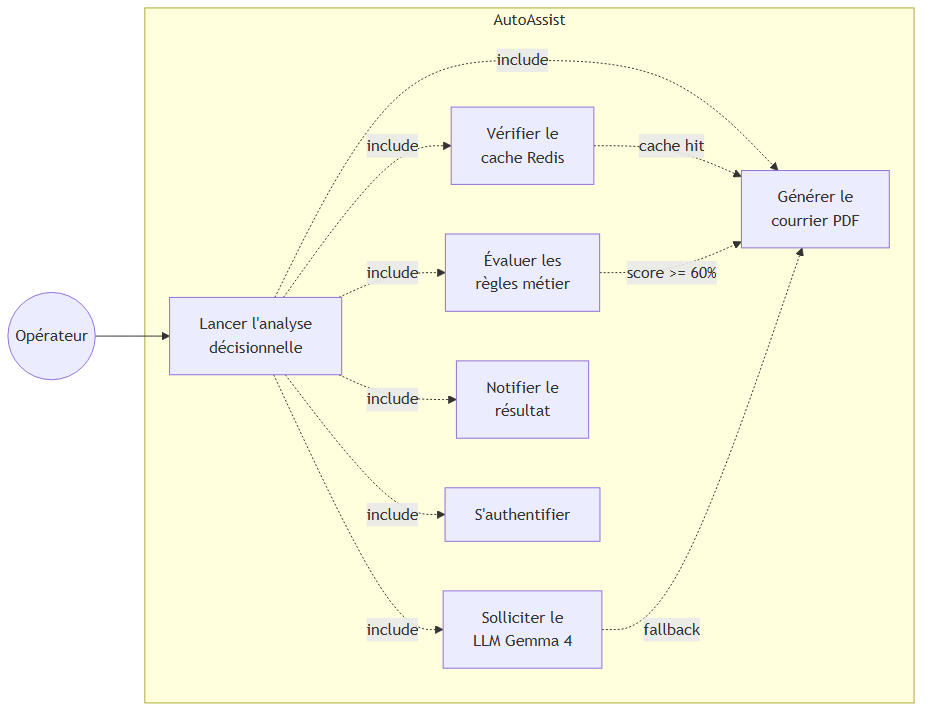
\includegraphics[width=0.80\textwidth]{figures/raffinement_decision.png}
    \caption{Raffinement du cas d'utilisation \og Traiter un ticket avec aide IA \fg{}}
    \label{fig:uc_decision}
\end{figure}

Le tableau~\ref{tab:uc_traiter} pr\'{e}sente la description textuelle du cas d'utilisation \og Traiter un ticket avec aide IA \fg{}.

\begin{table}[H]
\centering
\caption{Description textuelle du cas d'utilisation \og Traiter un ticket \fg{}}
\label{tab:uc_traiter}
\begin{tabular}{|p{3.5cm}|p{9.5cm}|}
\hline
\textbf{\'{E}l\'{e}ment} & \textbf{Description} \\
\hline
Cas d'utilisation & Traiter un ticket avec aide IA. \\
\hline
Acteur & Op\'{e}rateur \\
\hline
Objectif & Permettre \`{a} l'op\'{e}rateur de traiter une demande client en exploitant la transcription automatique, l'analyse NLP et le pipeline d\'{e}cisionnel hybride. \\
\hline
Pr\'{e}conditions & L'acteur doit \^{e}tre authentifi\'{e} dans l'application. Un ticket doit exister. \\
\hline
Postconditions & La d\'{e}cision est finalis\'{e}e, un courrier PDF est g\'{e}n\'{e}r\'{e} et le ticket est mis \`{a} jour. \\
\hline
Sc\'{e}nario nominal & 1. L'op\'{e}rateur s'authentifie sur l'application. \newline 2. Il ouvre le d\'{e}tail du ticket. \newline 3. Il uploade l'enregistrement audio. \newline 4. Whisper transcrit et spaCy analyse~: \newline \hspace{0.5cm} -- Extraction des mots-cl\'{e}s. \newline \hspace{0.5cm} -- D\'{e}tection du type de sinistre. \newline \hspace{0.5cm} -- Analyse du sentiment. \newline 5. Le formulaire est pr\'{e}-rempli. \newline 6. L'op\'{e}rateur lance l'analyse d\'{e}cisionnelle. \newline 7. Il accepte ou rejette la recommandation. \\
\hline
\end{tabular}
\end{table}

\subsubsection{Raffinement du cas d'utilisation \og Interroger le chatbot WhatsApp \fg{}}

La figure~\ref{fig:uc_chatbot} pr\'{e}sente le diagramme de cas d'utilisation raffin\'{e} du cas d'utilisation \og Interroger le chatbot WhatsApp \fg{}.

\begin{figure}[htbp]
    \centering
    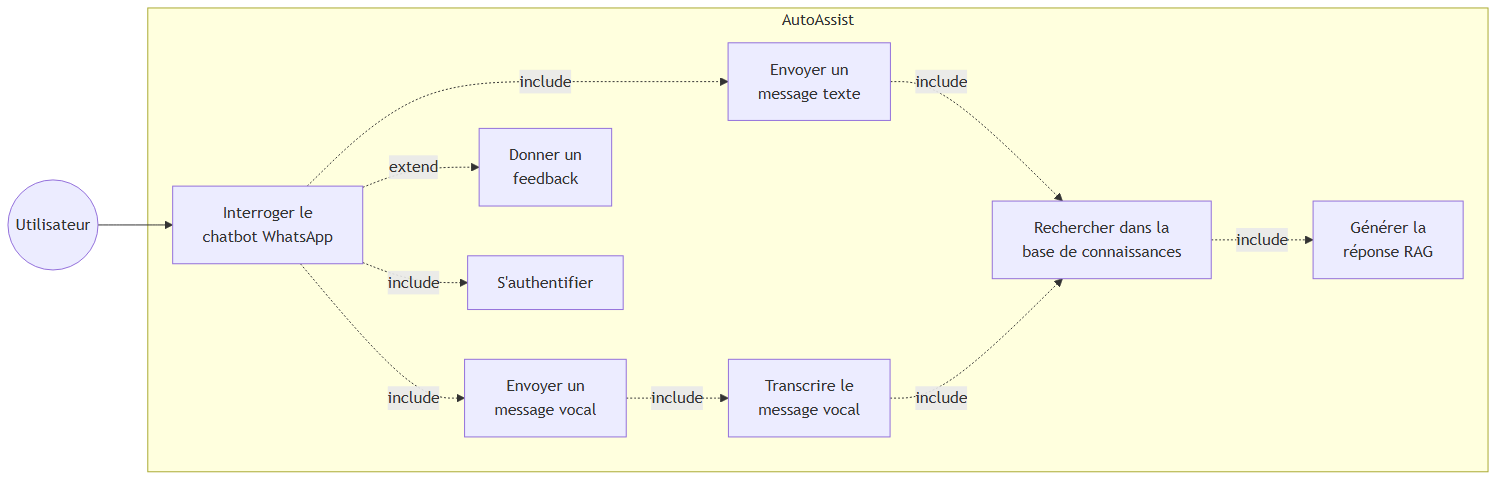
\includegraphics[width=\textwidth]{figures/raffinement_chatbot.png}
    \caption{Raffinement du cas d'utilisation \og Interroger le chatbot \fg{}}
    \label{fig:uc_chatbot}
\end{figure}

\begin{table}[H]
\centering
\caption{Description textuelle du cas d'utilisation \og Interroger le chatbot \fg{}}
\label{tab:uc_chatbot}
\begin{tabular}{|p{3.5cm}|p{9.5cm}|}
\hline
\textbf{\'{E}l\'{e}ment} & \textbf{Description} \\
\hline
Cas d'utilisation & Interroger le chatbot WhatsApp. \\
\hline
Acteur & Op\'{e}rateur / Superviseur \\
\hline
Objectif & Permettre aux utilisateurs d'obtenir des r\'{e}ponses pr\'{e}cises sur les proc\'{e}dures internes et les r\`{e}gles m\'{e}tier via un chatbot intelligent. \\
\hline
Pr\'{e}conditions & L'acteur doit \^{e}tre authentifi\'{e}. Le service RAG doit \^{e}tre op\'{e}rationnel. \\
\hline
Postconditions & Une r\'{e}ponse pertinente est envoy\'{e}e \`{a} l'utilisateur via WhatsApp. \\
\hline
Sc\'{e}nario nominal & 1. L'utilisateur envoie un message (texte ou vocal). \newline 2. Le syst\`{e}me identifie le type de message~: \newline \hspace{0.5cm} -- Message texte~: recherche hybride ChromaDB. \newline \hspace{0.5cm} -- Message vocal~: transcription Whisper puis RAG. \newline \hspace{0.5cm} -- Commande rapide~: ex\'{e}cution API directe. \newline 3. Le syst\`{e}me g\'{e}n\`{e}re et envoie la r\'{e}ponse. \\
\hline
\end{tabular}
\end{table}

\subsubsection{Raffinement du cas d'utilisation \og Configurer les r\`{e}gles d'assurance \fg{}}

La figure~\ref{fig:uc_rules_raff} pr\'{e}sente le diagramme de cas d'utilisation raffin\'{e} du cas d'utilisation \og Configurer les r\`{e}gles d'assurance \fg{}.

\begin{figure}[htbp]
    \centering
    \includegraphics[width=0.80\textwidth]{figures/raffinement_rules.png}
    \caption{Raffinement du cas d'utilisation \og Configurer les r\`{e}gles \fg{}}
    \label{fig:uc_rules_raff}
\end{figure}

\begin{table}[H]
\centering
\caption{Description textuelle du cas d'utilisation \og Configurer les r\`{e}gles \fg{}}
\label{tab:uc_rules}
\begin{tabular}{|p{3.5cm}|p{9.5cm}|}
\hline
\textbf{\'{E}l\'{e}ment} & \textbf{Description} \\
\hline
Cas d'utilisation & Configurer les r\`{e}gles d'assurance. \\
\hline
Acteur & Superviseur \\
\hline
Objectif & Permettre au superviseur de cr\'{e}er, modifier et tester des r\`{e}gles d'assurance via un \'{e}diteur visuel, incluant le versioning. \\
\hline
Pr\'{e}conditions & L'acteur doit \^{e}tre authentifi\'{e} dans l'application. \\
\hline
Postconditions & Les r\`{e}gles sont cr\'{e}\'{e}es, modifi\'{e}es ou activ\'{e}es selon les actions r\'{e}alis\'{e}es. L'historique de versioning est mis \`{a} jour. \\
\hline
Sc\'{e}nario nominal & 1. Le superviseur s'authentifie sur l'application. \newline 2. Il acc\`{e}de \`{a} l'\'{e}diteur visuel de r\`{e}gles. \newline 3. Il peut~: \newline \hspace{0.5cm} -- Cr\'{e}er une nouvelle r\`{e}gle (conditions JSONB). \newline \hspace{0.5cm} -- Modifier une r\`{e}gle existante. \newline \hspace{0.5cm} -- Tester avec des donn\'{e}es fictives. \newline \hspace{0.5cm} -- Activer ou d\'{e}sactiver une r\`{e}gle. \newline 4. Le syst\`{e}me enregistre et versionne la r\`{e}gle. \\
\hline
\end{tabular}
\end{table}

\section{Cadre m\'{e}thodologique}
\label{sec:cadre}

\subsection{M\'{e}thodologie de d\'{e}veloppement~: Scrum}

Une m\'{e}thodologie de d\'{e}veloppement logiciel d\'{e}finit les diff\'{e}rentes \'{e}tapes et s\'{e}quences dans le processus de r\'{e}alisation d'une application. Face \`{a} la complexit\'{e} croissante des projets informatiques et \`{a} la n\'{e}cessit\'{e} de s'adapter rapidement aux \'{e}volutions des besoins, les approches agiles se sont impos\'{e}es comme une alternative plus flexible aux m\'{e}thodes traditionnelles de gestion de projet.

\indent Parmi les m\'{e}thodes de d\'{e}veloppement classiques, le \textbf{cycle en V} garantit une documentation exhaustive et une tra\c{c}abilit\'{e} rigoureuse des exigences, mais il pr\'{e}sente l'inconv\'{e}nient majeur de livrer le produit final en une seule fois, \`{a} la fin du projet. Toute erreur de conception d\'{e}tect\'{e}e tardivement engendre alors un co\^{u}t de correction \'{e}lev\'{e}. De m\^{e}me, \textbf{Kanban} offre une gestion visuelle efficace du flux de t\^{a}ches, mais sans cadre temporel d\'{e}fini ni m\'{e}canisme de planification des incr\'{e}ments fonctionnels.

\indent \textbf{Scrum}, en revanche, est un cadre de travail agile qui permet de relever ces d\'{e}fis en organisant le d\'{e}veloppement autour de cycles courts et it\'{e}ratifs appel\'{e}s \textit{sprints} \cite{scrum}. Il repose sur trois piliers fondamentaux~: la \textbf{transparence}, qui impose que les aspects significatifs du processus soient visibles de tous les acteurs concern\'{e}s~; l'\textbf{inspection}, qui exige une \'{e}valuation fr\'{e}quente des artefacts et de la progression vers les objectifs~; et l'\textbf{adaptation}, qui permet d'ajuster le processus d\`{e}s qu'un \'{e}cart est d\'{e}tect\'{e}.

\indent Chaque sprint, d'une dur\'{e}e fixe de deux \`{a} quatre semaines, comprend une phase de planification (\textit{Sprint Planning}), des r\'{e}unions quotidiennes de synchronisation (\textit{Daily Scrum}), une revue des fonctionnalit\'{e}s livr\'{e}es (\textit{Sprint Review}) et une r\'{e}trospective collective (\textit{Sprint Retrospective}).

\indent \textbf{Justification du choix de Scrum pour AutoAssist.} Le projet AutoAssist pr\'{e}sente plusieurs caract\'{e}ristiques qui rendent Scrum particuli\`{e}rement adapt\'{e}. D'une part, la complexit\'{e} technique est \'{e}lev\'{e}e~: onze microservices ind\'{e}pendants, trois langages de programmation (Java, Python, Dart) et plusieurs technologies d'IA (Whisper, spaCy, Gemma~4, RAG) impliquent des interd\'{e}pendances nombreuses qu'il est pr\'{e}f\'{e}rable de valider par it\'{e}rations successives plut\^{o}t que de sp\'{e}cifier exhaustivement en amont. D'autre part, certaines fonctionnalit\'{e}s --- notamment le pipeline d\'{e}cisionnel hybride et le chatbot WhatsApp --- n\'{e}cessitent des retours utilisateur r\'{e}guliers pour affiner les param\`{e}tres des mod\`{e}les IA et les seuils de d\'{e}cision. Enfin, la m\'{e}thode Scrum facilite la communication entre l'\'{e}quipe de d\'{e}veloppement et les parties prenantes m\'{e}tier, garantissant un alignement continu entre les fonctionnalit\'{e}s livr\'{e}es et les besoins r\'{e}els du terrain.

\subsection{Pilotage du projet par Scrum}

Pour le projet AutoAssist, les r\^{o}les Scrum sont attribu\'{e}s comme suit~:

\begin{itemize}[label=---]
    \item \textbf{M. Nezar Torche~:} Il occupe le r\^{o}le de Product Owner. En tant que principal point de contact au sein de l'entreprise, il d\'{e}finit les besoins et priorit\'{e}s du projet, g\`{e}re le Product Backlog et valide les livrables.
    \item \textbf{Mme Hedia Selmi~:} Elle joue le r\^{o}le de Scrum Master. En tant qu'encadreur professionnel, elle veille \`{a} la bonne application de la d\'{e}marche Scrum, facilite les r\'{e}unions et aide \`{a} la r\'{e}solution des obstacles rencontr\'{e}s par l'\'{e}quipe.
    \item \textbf{Rezgui Seif Eddine~:} Il joue le r\^{o}le d'un membre de l'\'{E}quipe de D\'{e}veloppement. Responsable de l'ex\'{e}cution des t\^{a}ches, du d\'{e}veloppement des fonctionnalit\'{e}s et de la livraison des incr\'{e}ments du produit \`{a} la fin de chaque Sprint. Il assure la conception, la r\'{e}alisation technique et la qualit\'{e} des fonctionnalit\'{e}s d\'{e}velopp\'{e}es.
\end{itemize}

\subsection{Backlog du produit}

Cette section met en lumi\`{e}re l'\'{e}l\'{e}ment central de la planification~: le backlog produit. Le tableau~\ref{tab:backlog} en pr\'{e}sente une version structur\'{e}e, regroupant l'ensemble des fonctionnalit\'{e}s dans notre projet.

\begin{longtable}{|c|p{2.5cm}|c|p{5.8cm}|c|}
\caption{Backlog du produit} \label{tab:backlog} \\
\hline
\textbf{ID-F} & \textbf{Features} & \textbf{ID-Us} & \textbf{User Stories} & \textbf{Priorit\'{e}} \\
\hline
\endfirsthead
\hline \textbf{ID-F} & \textbf{Features} & \textbf{ID-Us} & \textbf{User Stories} & \textbf{Priorit\'{e}} \\ \hline
\endhead
\multirow{2}{*}{1} & \multirow{2}{2.8cm}{Authentification} & 1.1 & En tant qu'utilisateur, je souhaite m'authentifier afin d'acc\'{e}der \`{a} la plateforme. & Haute \\
\cline{3-5}
 & & 1.2 & En tant qu'utilisateur, je souhaite pouvoir me d\'{e}connecter pour s\'{e}curiser mon compte. & Moyenne \\
\hline
\multirow{3}{*}{2} & \multirow{3}{2.8cm}{Gestion des utilisateurs et agences} & 2.1 & En tant qu'admin, je souhaite g\'{e}rer les utilisateurs en cr\'{e}ant des comptes et en attribuant les r\^{o}les. & Haute \\
\cline{3-5}
 & & 2.2 & En tant qu'admin, je souhaite g\'{e}rer les agences afin d'organiser la structure de l'entreprise. & Haute \\
\cline{3-5}
 & & 2.3 & En tant qu'utilisateur, je souhaite consulter et modifier mon profil. & Moyenne \\
\hline
\multirow{3}{*}{3} & \multirow{3}{2.8cm}{Gestion des tickets} & 3.1 & En tant qu'op\'{e}rateur, je souhaite cr\'{e}er un ticket \`{a} partir d'un appel, email ou formulaire. & Haute \\
\cline{3-5}
 & & 3.2 & En tant qu'op\'{e}rateur, je souhaite suivre le cycle de vie d'un ticket en temps r\'{e}el. & Haute \\
\cline{3-5}
 & & 3.3 & En tant que client, je souhaite soumettre ma demande via un formulaire web. & Moyenne \\
\hline
\multirow{2}{*}{4} & \multirow{2}{2.8cm}{Transcription et analyse IA} & 4.1 & En tant qu'op\'{e}rateur, je souhaite transcrire un enregistrement audio afin d'obtenir le texte de l'appel. & Haute \\
\cline{3-5}
 & & 4.2 & En tant que syst\`{e}me, je souhaite pr\'{e}-remplir le formulaire avec les donn\'{e}es extraites par NLP. & Haute \\
\hline
\multirow{2}{*}{5} & \multirow{2}{2.8cm}{Pipeline d\'{e}cisionnel} & 5.1 & En tant qu'op\'{e}rateur, je souhaite lancer l'analyse d\'{e}cisionnelle afin d'obtenir une recommandation. & Haute \\
\cline{3-5}
 & & 5.2 & En tant qu'op\'{e}rateur, je souhaite g\'{e}n\'{e}rer un courrier PDF apr\`{e}s la d\'{e}cision. & Haute \\
\hline
\multirow{2}{*}{6} & \multirow{2}{2.8cm}{Chatbot WhatsApp} & 6.1 & En tant qu'utilisateur, je souhaite interroger le chatbot sur les proc\'{e}dures internes. & Haute \\
\cline{3-5}
 & & 6.2 & En tant qu'utilisateur, je souhaite envoyer un message vocal au chatbot. & Moyenne \\
\hline
7 & R\`{e}gles m\'{e}tier & 7.1 & En tant que superviseur, je souhaite configurer les r\`{e}gles d'assurance via un \'{e}diteur visuel. & Haute \\
\hline
8 & Analytics & 8.1 & En tant que superviseur, je souhaite consulter les KPIs et tableaux de bord. & Moyenne \\
\hline
9 & Mobile & 9.1 & En tant qu'op\'{e}rateur, je souhaite g\'{e}rer les tickets depuis l'application mobile. & Basse \\
\hline
\end{longtable}

\subsection{Planification du projet avec sprints}

La planification des sprints constitue une \'{e}tape cl\'{e} dans l'organisation du d\'{e}veloppement du projet selon la m\'{e}thodologie Scrum. Pour garantir une progression structur\'{e}e et ma\^{i}tris\'{e}e, le projet a \'{e}t\'{e} d\'{e}coup\'{e} en six sprints successifs. Chaque sprint cible un ensemble coh\'{e}rent de fonctionnalit\'{e}s.

\indent Le d\'{e}coupage du projet se fait comme suit~:

\begin{table}[H]
\centering
\caption{Planification des sprints}
\label{tab:sprints}
\small
\begin{tabular}{|c|c|p{7cm}|c|}
\hline
\textbf{Sprint} & \textbf{Dur\'{e}e} & \textbf{Objectifs} & \textbf{ID-Us} \\
\hline
Sprint 0 & 3 sem. & Infrastructure, CI/CD et authentification & 1.1, 1.2 \\
\hline
Sprint 1 & 3 sem. & Organisations, tickets et canaux d'acquisition & 2.1--3.3 \\
\hline
Sprint 2 & 3 sem. & Service IA (transcription, NLP) et frontend & 4.1, 4.2 \\
\hline
Sprint 3 & 3 sem. & Moteur de r\`{e}gles, pipeline d\'{e}cisionnel, PDF & 5.1, 5.2, 7.1 \\
\hline
Sprint 4 & 3 sem. & Chatbot WhatsApp RAG et analytics & 6.1, 6.2, 8.1 \\
\hline
Sprint 5 & 2 sem. & Application mobile Flutter et tests & 9.1 \\
\hline
\end{tabular}
\end{table}

\section*{Conclusion}
\label{sec:conclusion}

Ce chapitre a permis d'analyser les besoins du projet, d'identifier les diff\'{e}rents acteurs, ainsi que de sp\'{e}cifier les besoins fonctionnels et non fonctionnels. Ces \'{e}l\'{e}ments ont \'{e}t\'{e} mod\'{e}lis\'{e}s \`{a} travers des diagrammes UML. La m\'{e}thodologie Scrum a structur\'{e} la planification en sprints pour une gestion agile et efficace. Le chapitre suivant se penchera sur la conception de la solution.

